\chapter{Axelrod's Model}\label{ch:1}

\resp{Bains, Arman Singh}

% \emph{
% Structure as\footnote{Remove this part from the report}:
% \begin{itemize}
% \item A short (max 1 page) explanation of the task, including references. Include mathematical concepts.
% \item Max 2 pages for the whole task (including figures)
% \item It is possible to use appendices for supplementary material, at the end of the report. Max 5 pages per task
% \end{itemize}
% A total of 3 pages + 5 supplementary pages per task
% }

\section{Introduction}
 
% Reference examples: book~\cite{barrat2008dynamical}, article~\cite{de2013mathematical}, website~\cite{weforumProtectingCritical}

% \section{Another section...}

% \lipsum[2-4]

% \lipsum[2-4]
% \lipsum[2-4]
% \lipsum[2-4]
% \lipsum[2-4]
% \lipsum[2-4]

The goal of Axelrod's model \cite{axelrod_dissemination_1997} hereby discussed is to explain why and how distinct cultural differences may persist, despite the interactions among individuals which should bring homogeneity since its expected that interacting individuals will eventually become more alike. The model proposes an agent-based adaptive model that should show how local convergence may indeed lead to global polarization or homogeneity.  \\
In this report, Axelrod's model will be firstly implemented on a lattice, in which nodes interact with their neighbors assimilating into their culture, possibly leading to a giant connected component in which all nodes have the same cultural characteristics. Then, the model will be also applied to different network topologies to see if there are similarities in how such a giant connected component emerges. Finally, in appendix \ref{ch:app1} a slightly different model will be presented, showing how an external force might affect the results which were previously obtained only for a decentralized model.

\section{Dynamics}
The basic model is implemented via a 10-by-10 lattice, in which each node is connected to its immediate neighbors (though free boundary conditions have been applied at the boundaries). To each node is assigned a culture, represented abstractly by a set of integer numbers. The size of the set is equal to the number of cultural features being examined (e.g. language, religion, etc.), while each integer number represents the specific cultural trait of the respective feature (e.g. italian or hindi for language). For the models described in this report, the initial cultural traits are assigned to each node by sampling from a uniform distribution. Cultural similarity among two neighbors is computed as the percentage of the features that have identical trait. \\
The process of social influence start by picking at random a node to be active, and then one of its neighbors. These two nodes interact with probability equal to their cultural similarity, with the active site copying one of the other's features.  \\
With only five distinct cultural traits and features, it seems that a giant connected component arises in a relatively small number of iterations ($\sim 10^5$) as can be seen in figure \ref{fig:ax}.

% \begin{figure}[ht]
%     \centering
%     \begin{subfigure}[t]{0.2\textwidth}
%         \centering
%         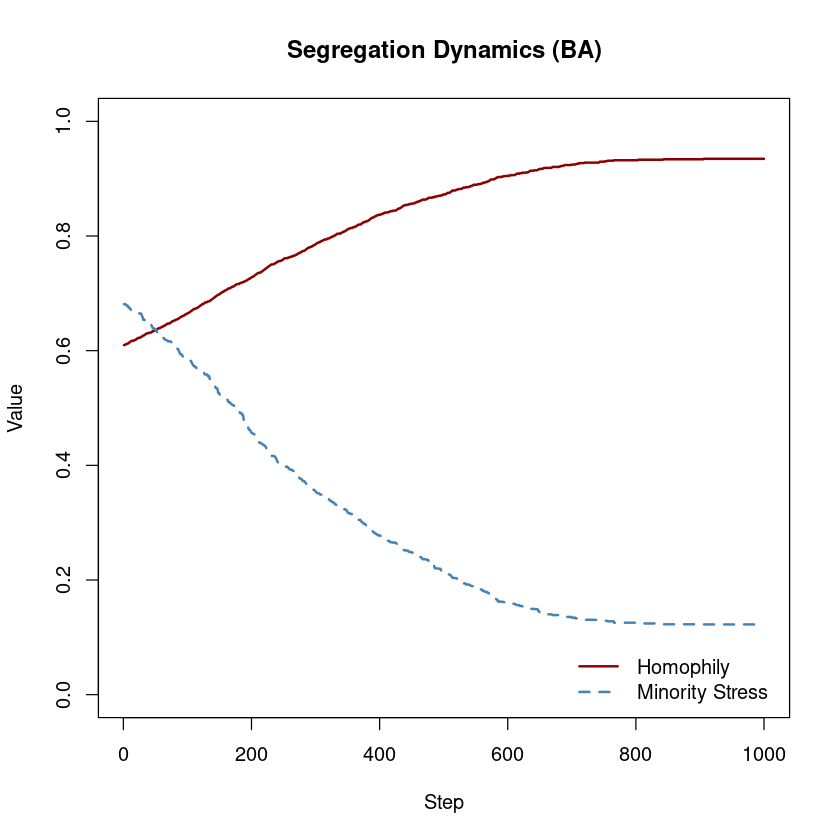
\includegraphics[width=\linewidth]{images/henryba.png}
%         \caption{Caption 1}
%     \end{subfigure}
%     \hfill
%     \begin{subfigure}[t]{0.2\textwidth}
%         \centering
%         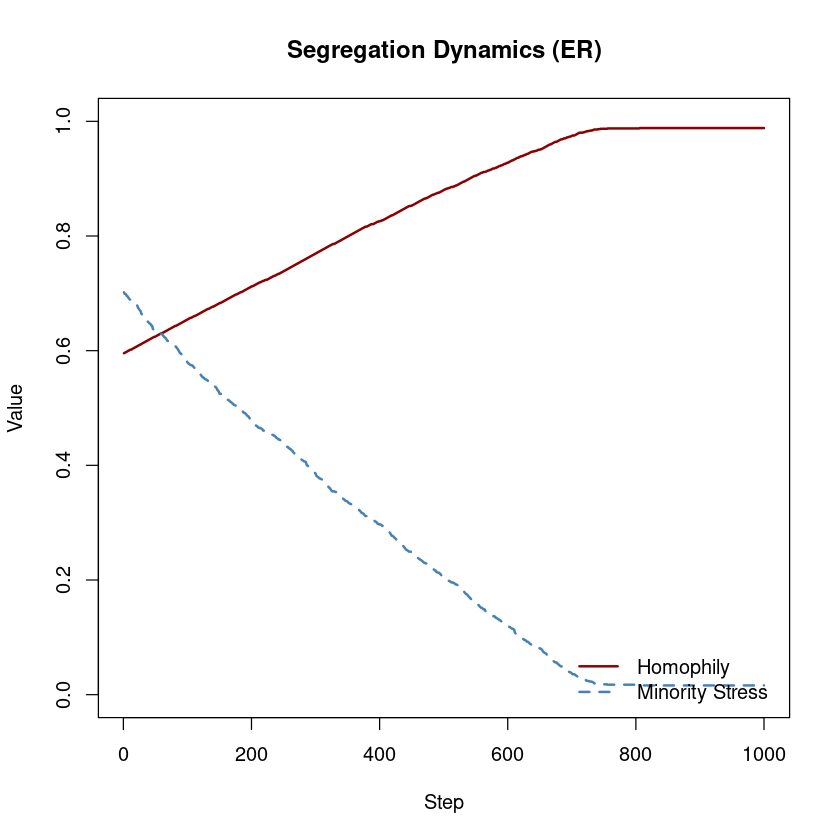
\includegraphics[width=\linewidth]{images/henryer.png}
%         \caption{Caption 2}
%     \end{subfigure}
%     \hfill
%     \begin{subfigure}[t]{0.2\textwidth}
%         \centering
%         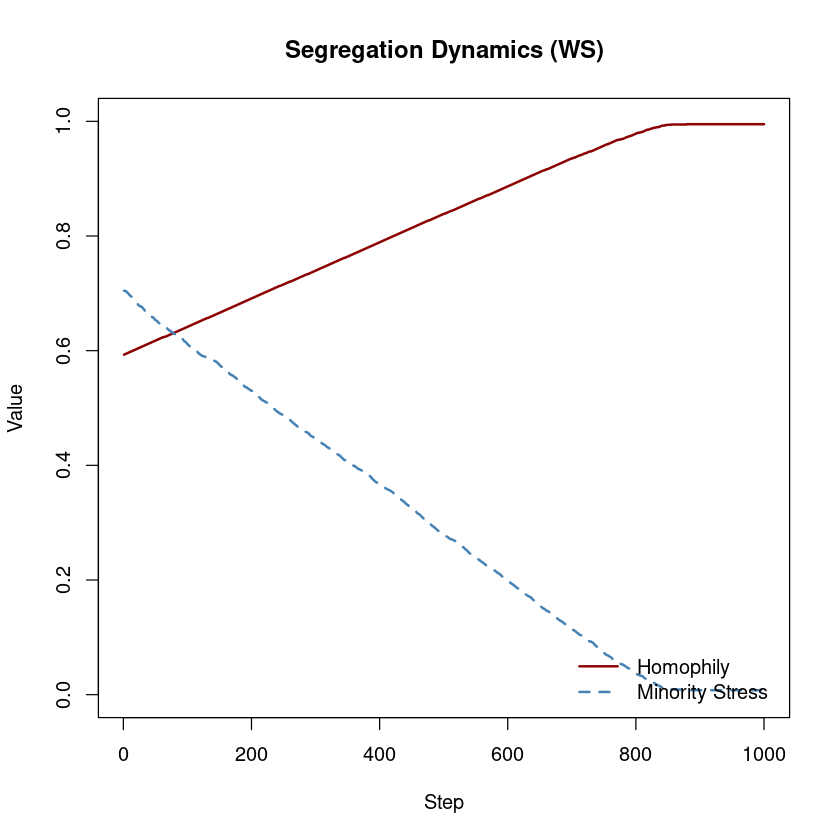
\includegraphics[width=\linewidth]{images/henryws.png}
%         \caption{Caption 3}
%     \end{subfigure}
%     \hfill
%     \begin{subfigure}[t]{0.2\textwidth}
%         \centering
%         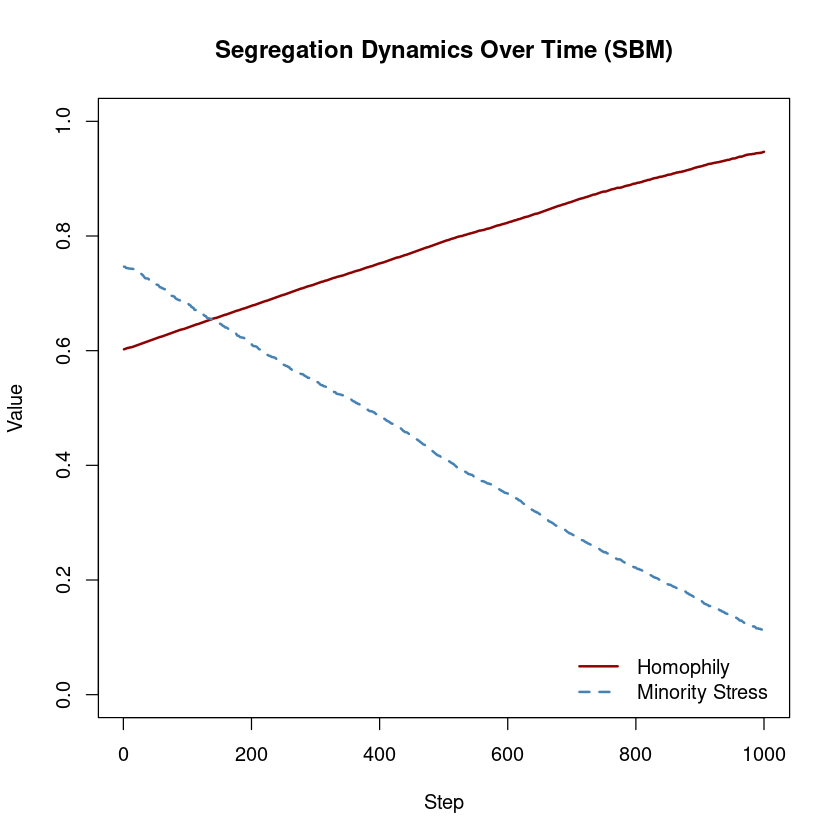
\includegraphics[width=\linewidth]{images/henrysbm.png}
%         \caption{Caption 4}
%     \end{subfigure}
%     \caption{Overall figure caption}
%     \label{fig:henry}
% \end{figure}




\begin{figure}[htbp]
    \centering
    \begin{minipage}[t]{0.24\linewidth}
        \centering
        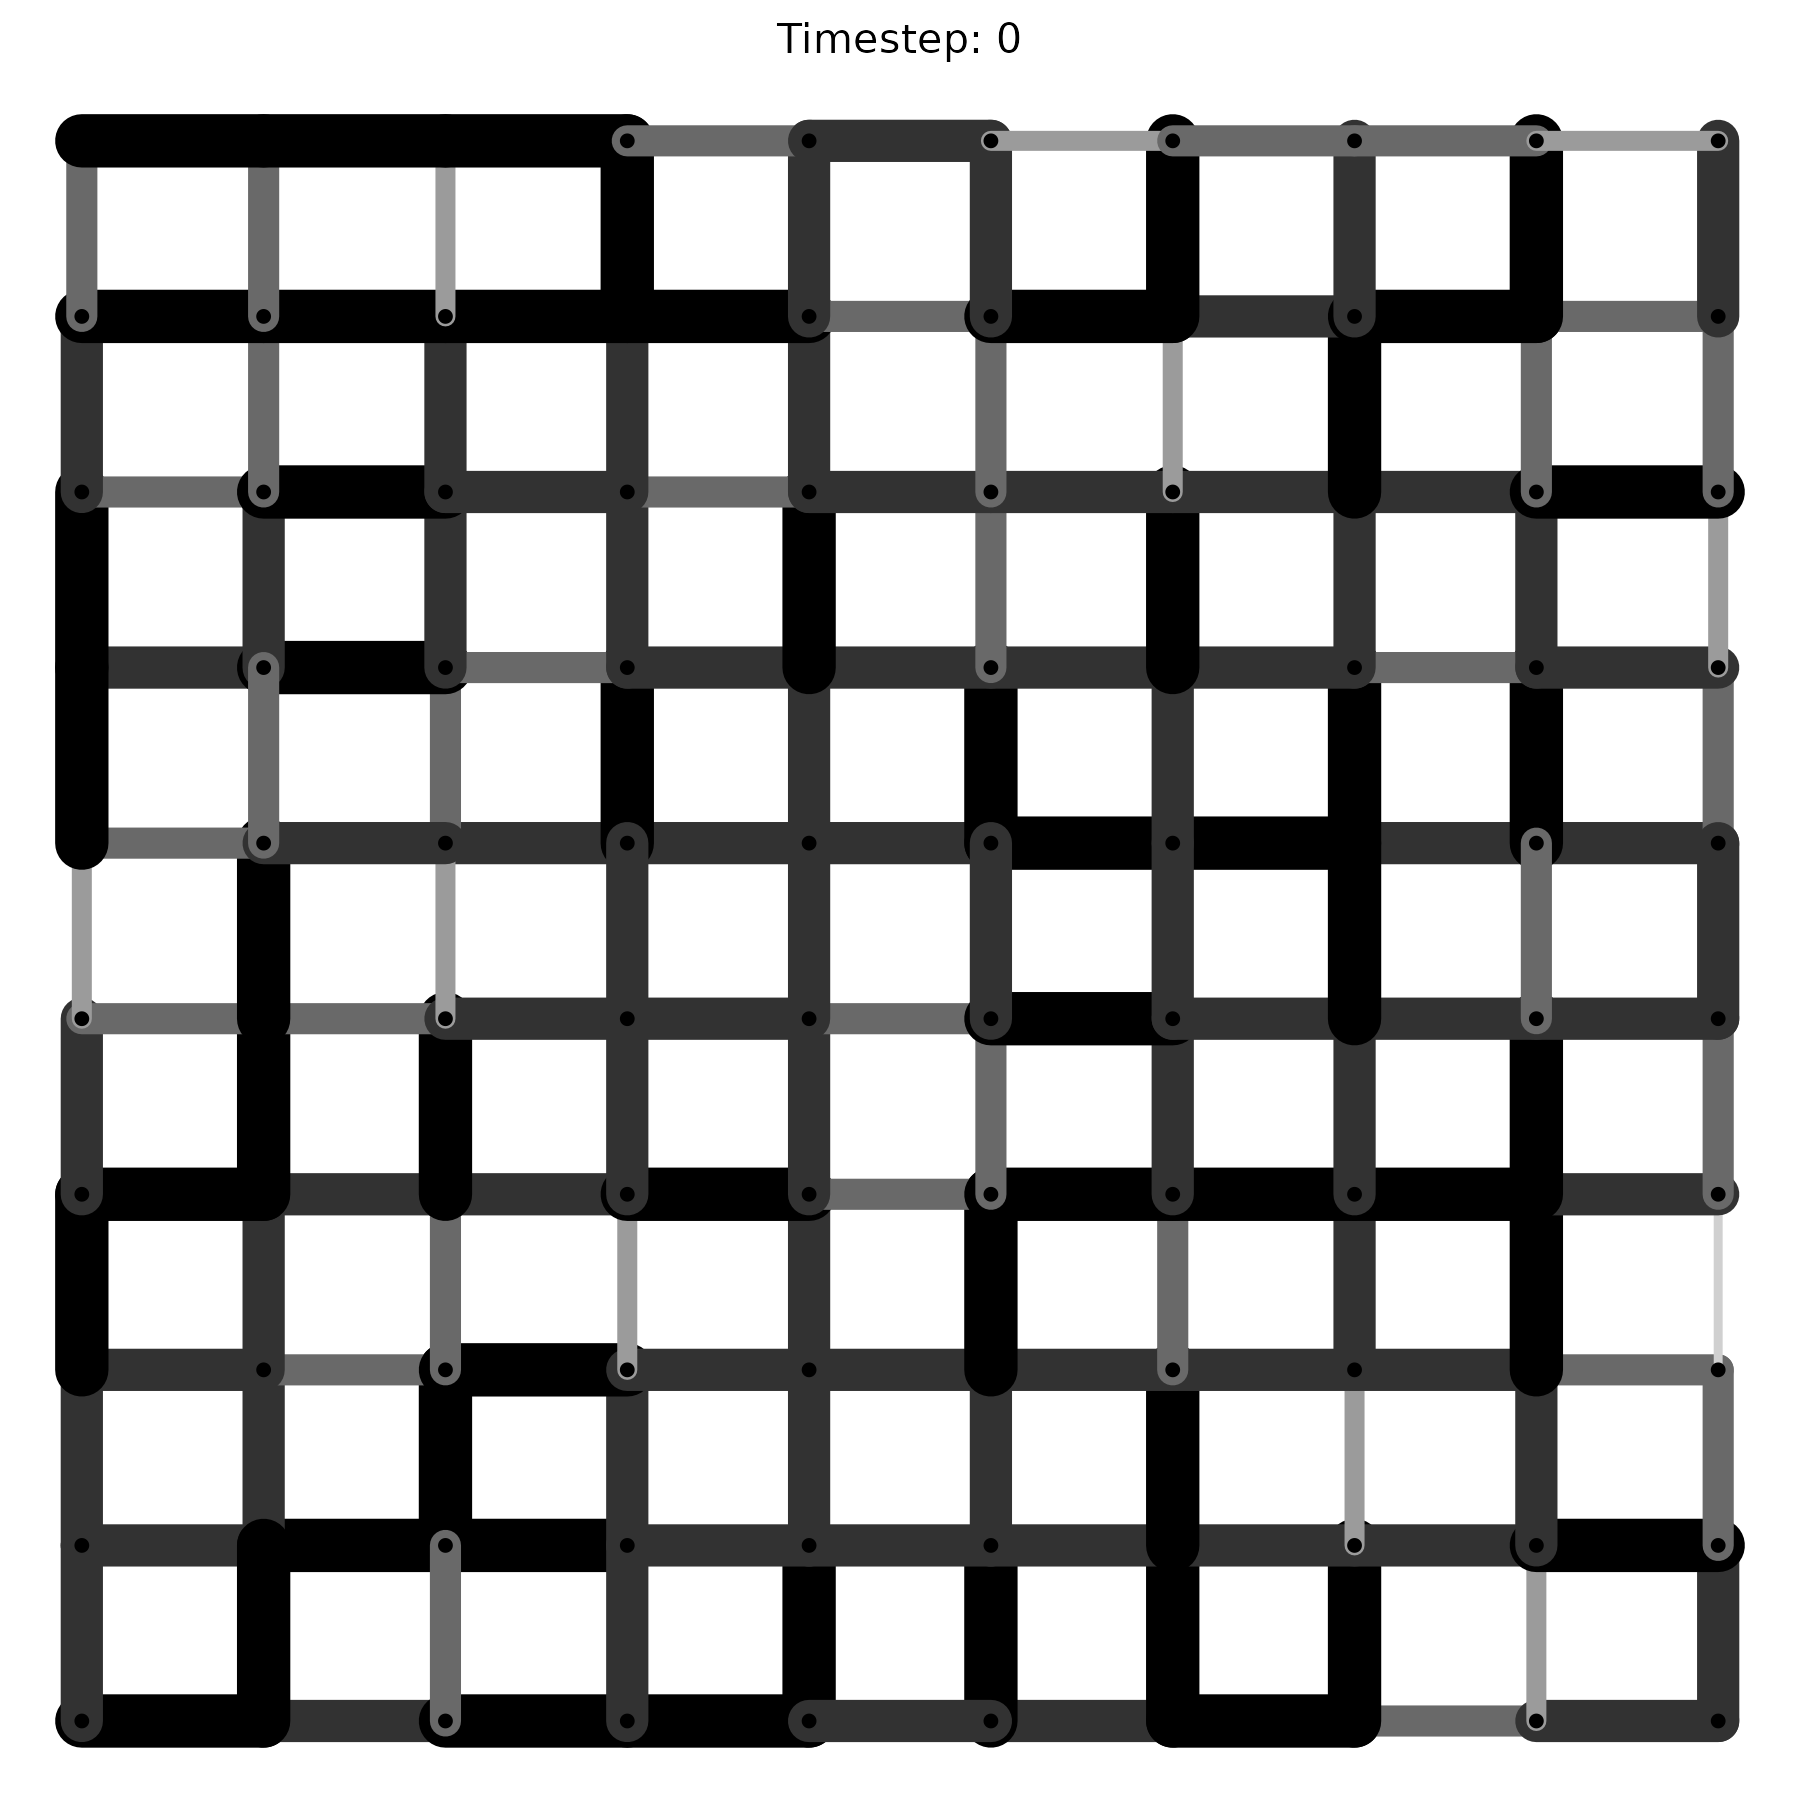
\includegraphics[width=\linewidth]{images/ax0.png}
        
    \end{minipage}
    \hfill
    \begin{minipage}[t]{0.24\linewidth}
        \centering
        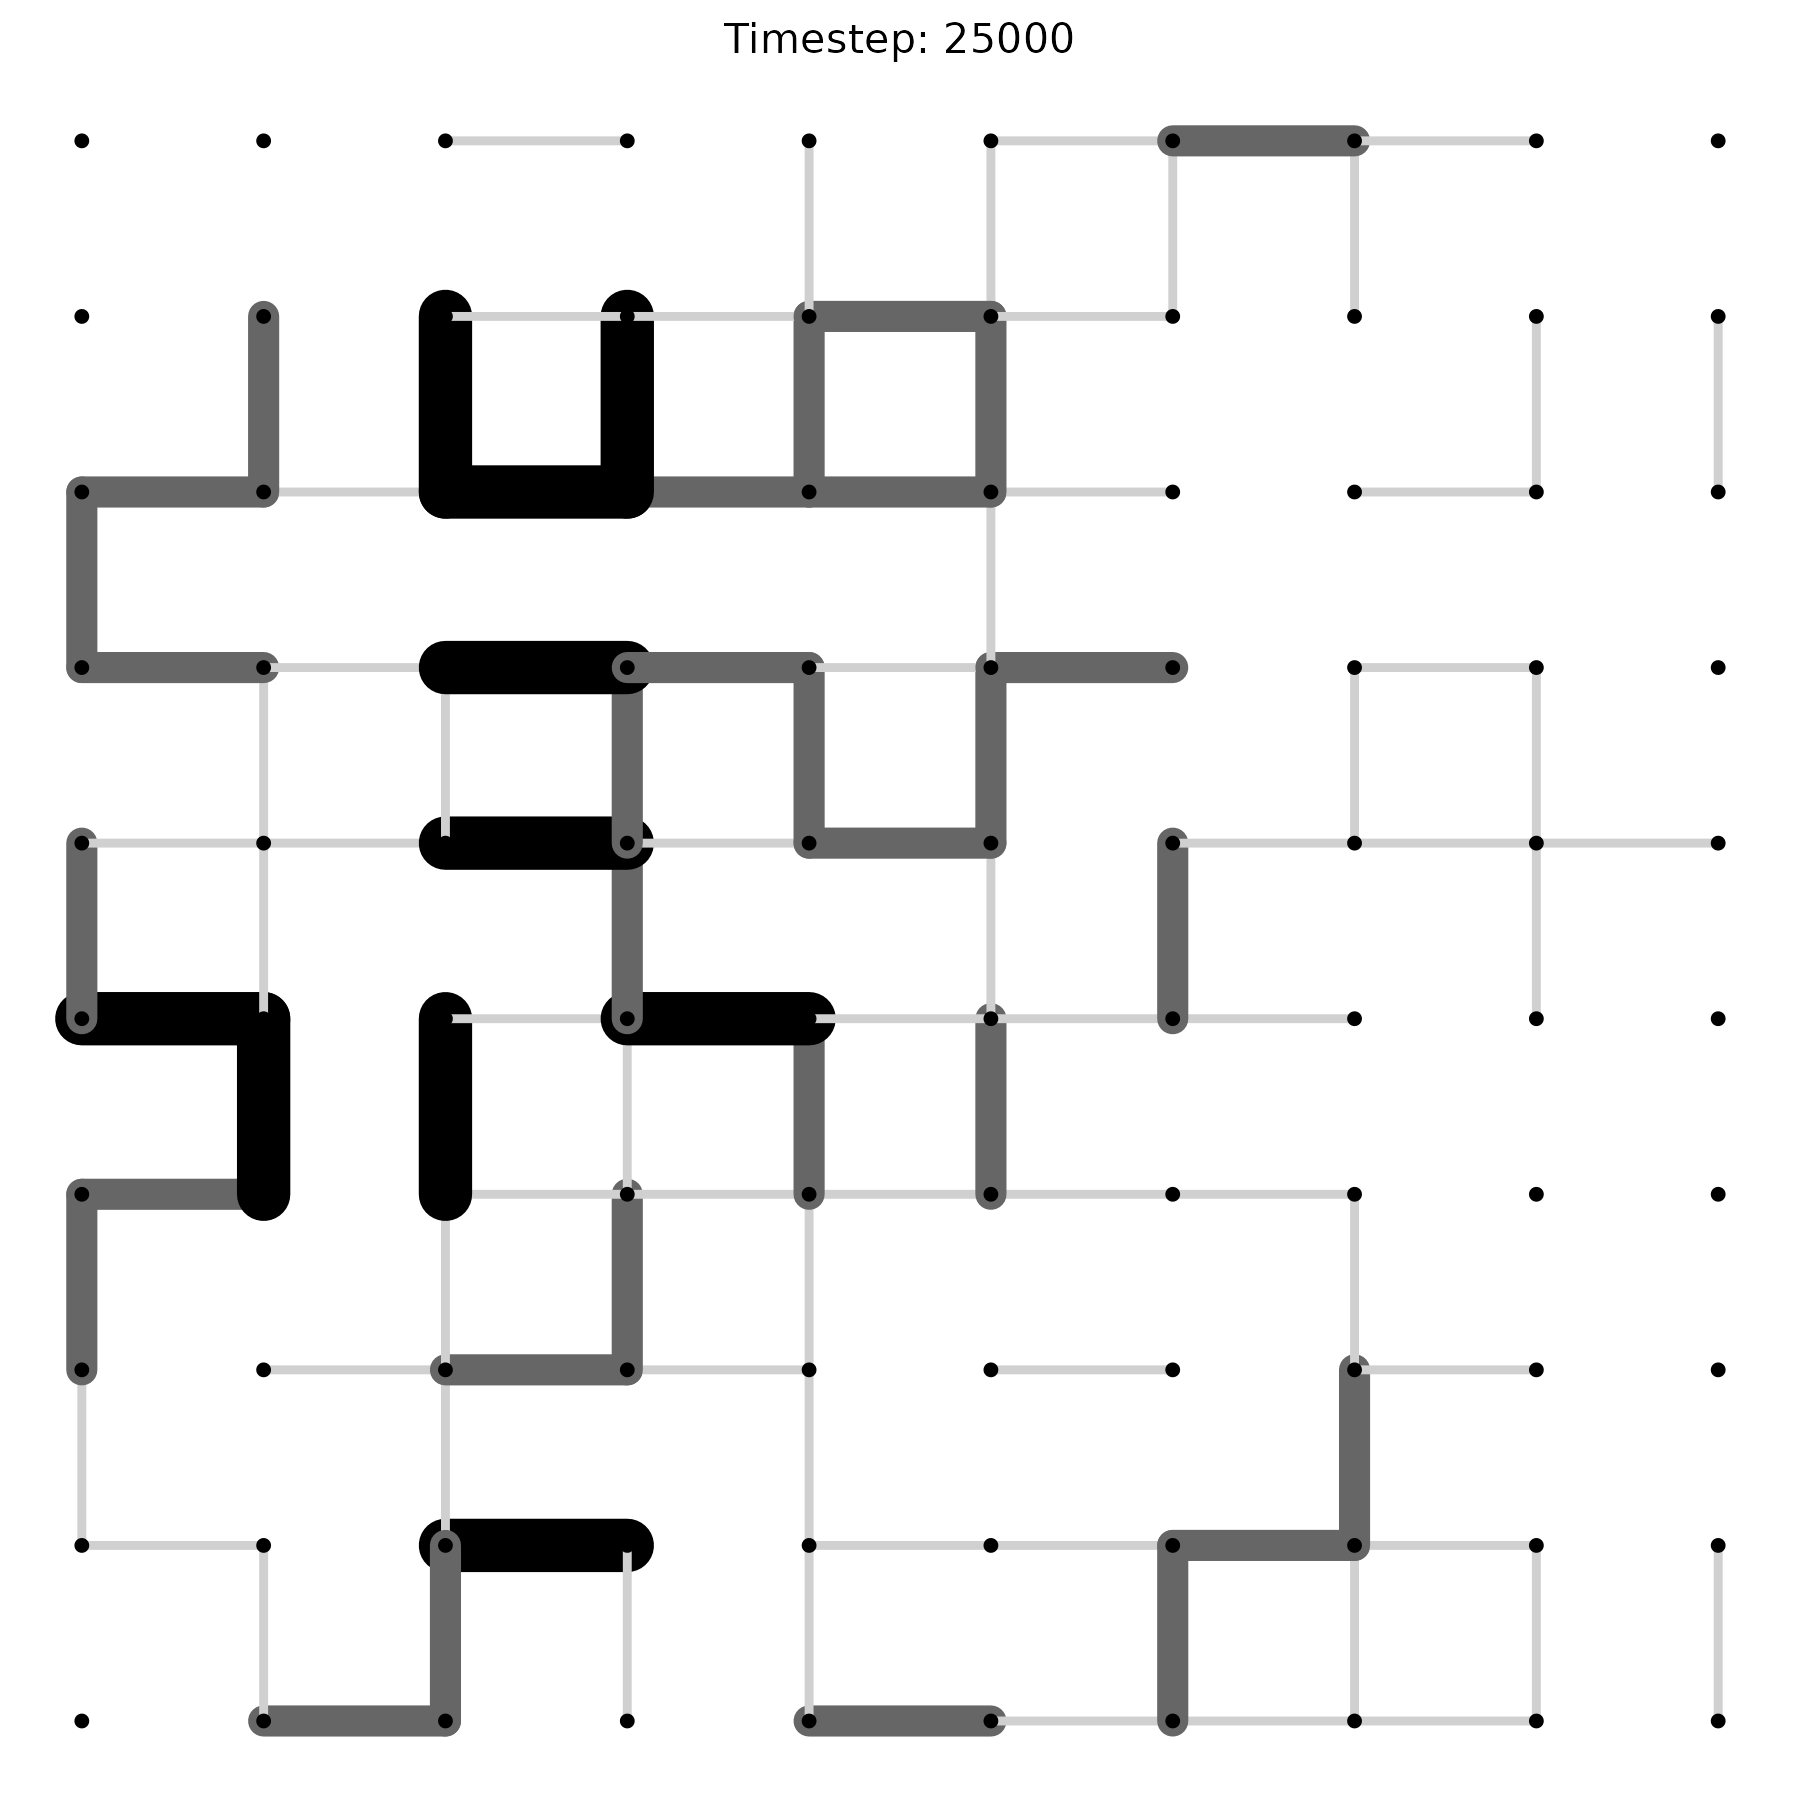
\includegraphics[width=\linewidth]{images/ax1.png}
        
    \end{minipage}
    \hfill
    \begin{minipage}[t]{0.24\linewidth}
        \centering
        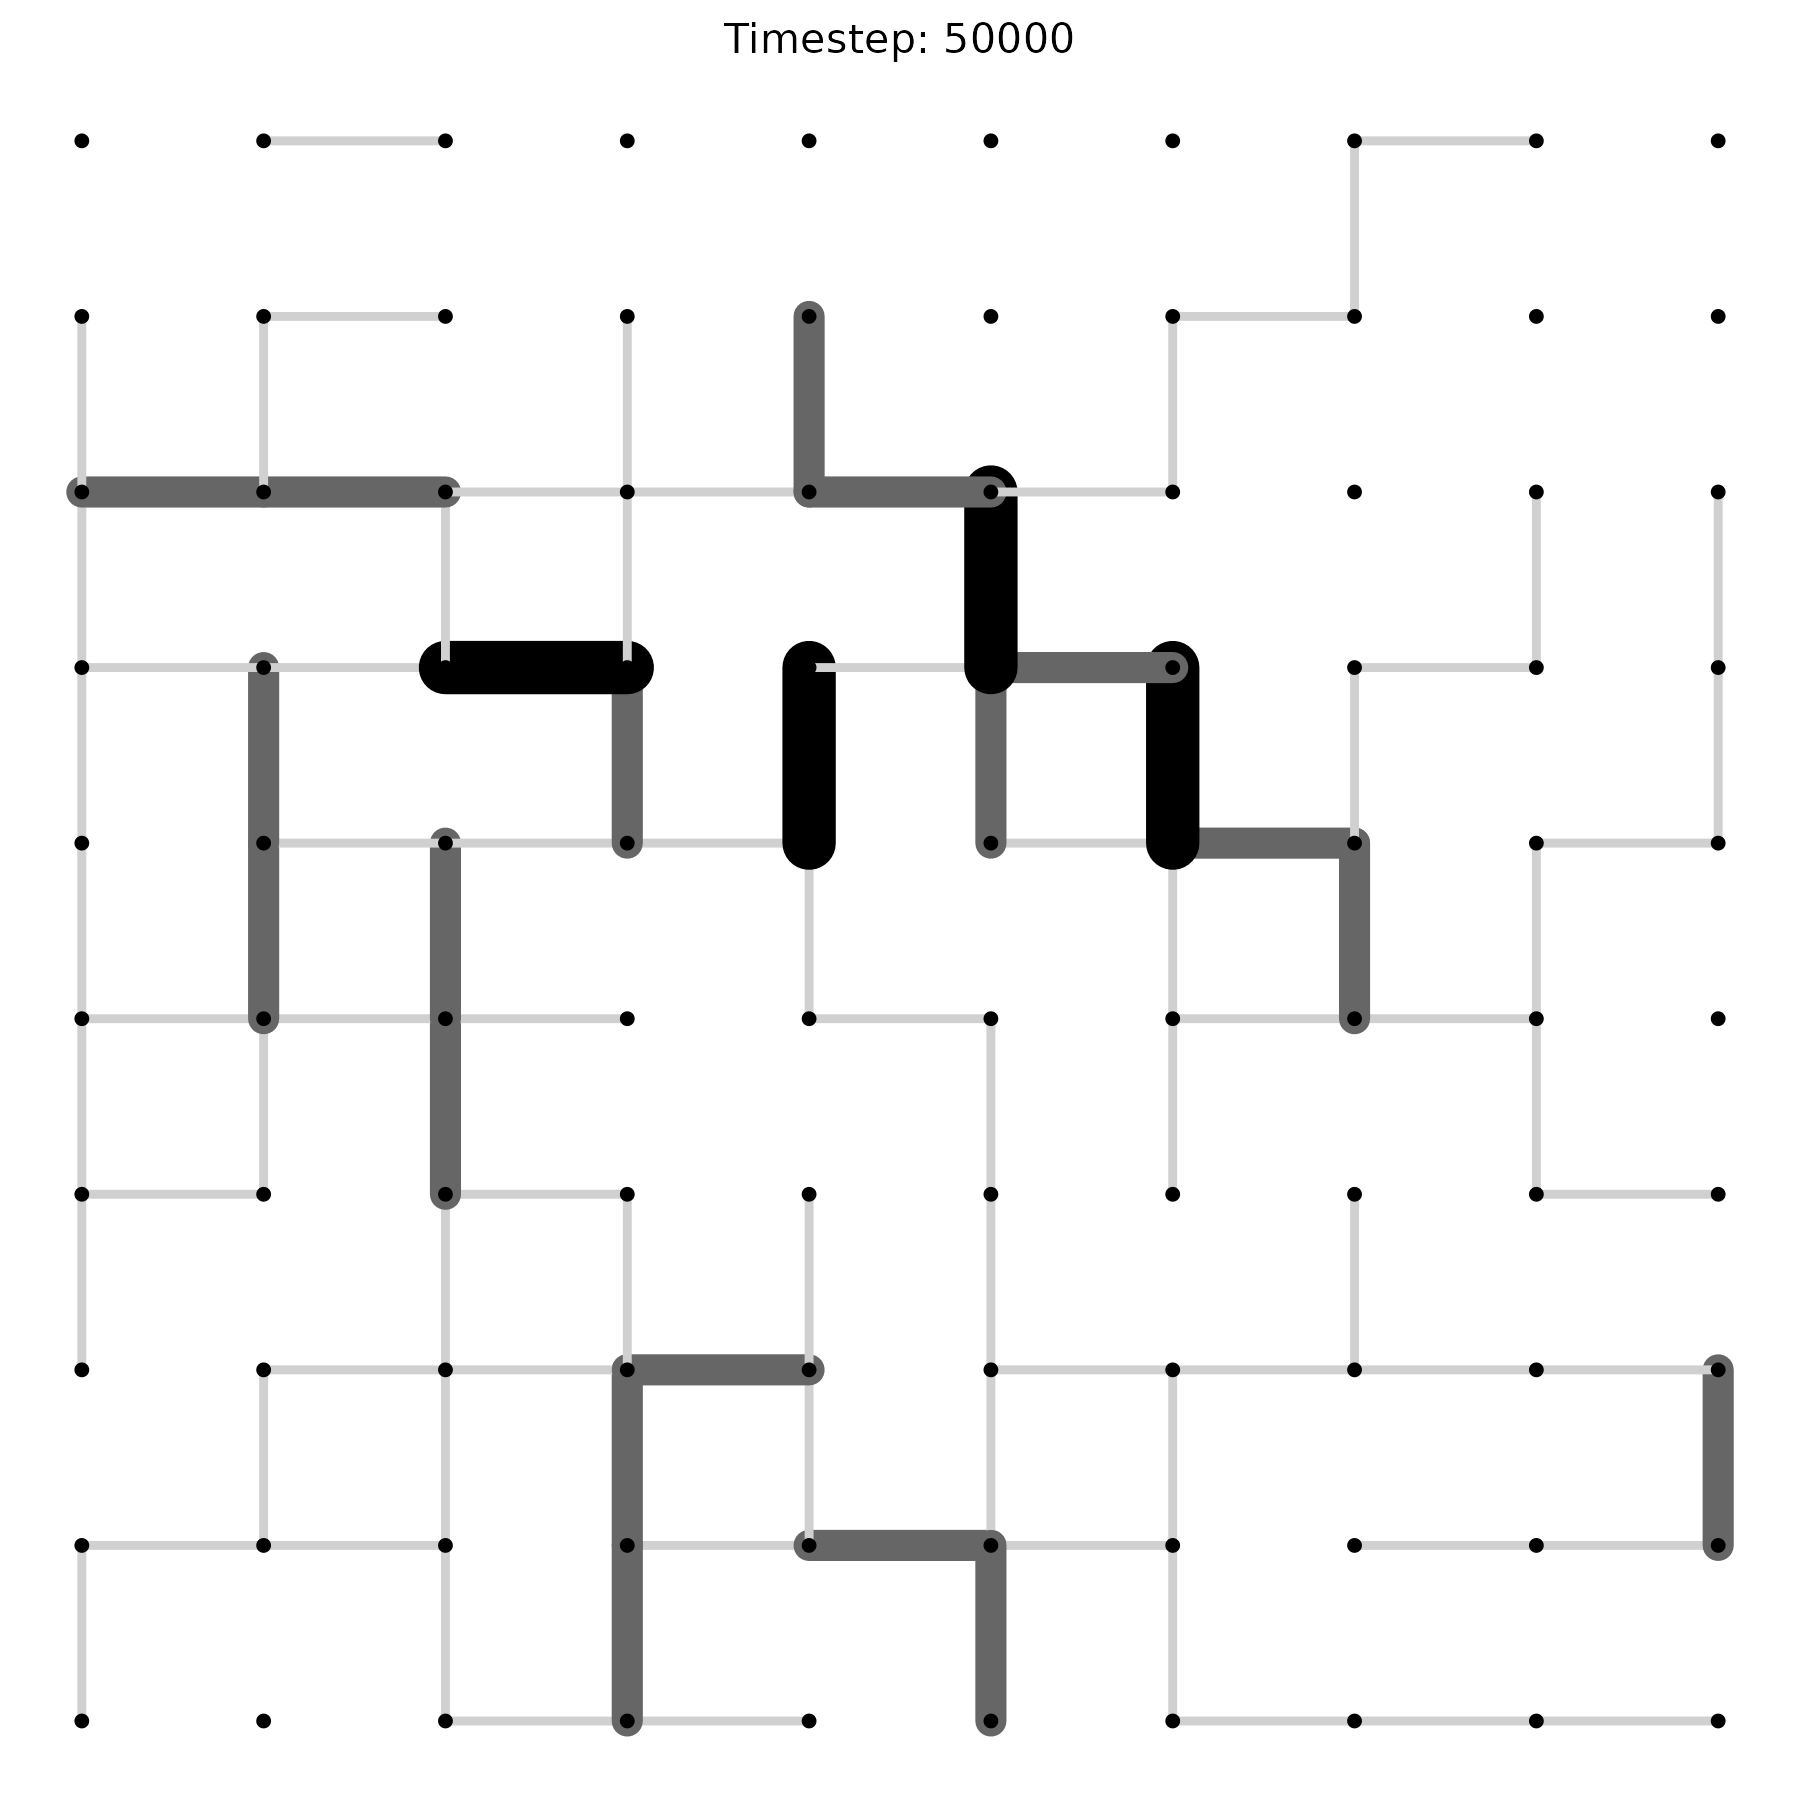
\includegraphics[width=\linewidth]{images/ax2.png}
        
    \end{minipage}
    \hfill
    \begin{minipage}[t]{0.24\linewidth}
        \centering
        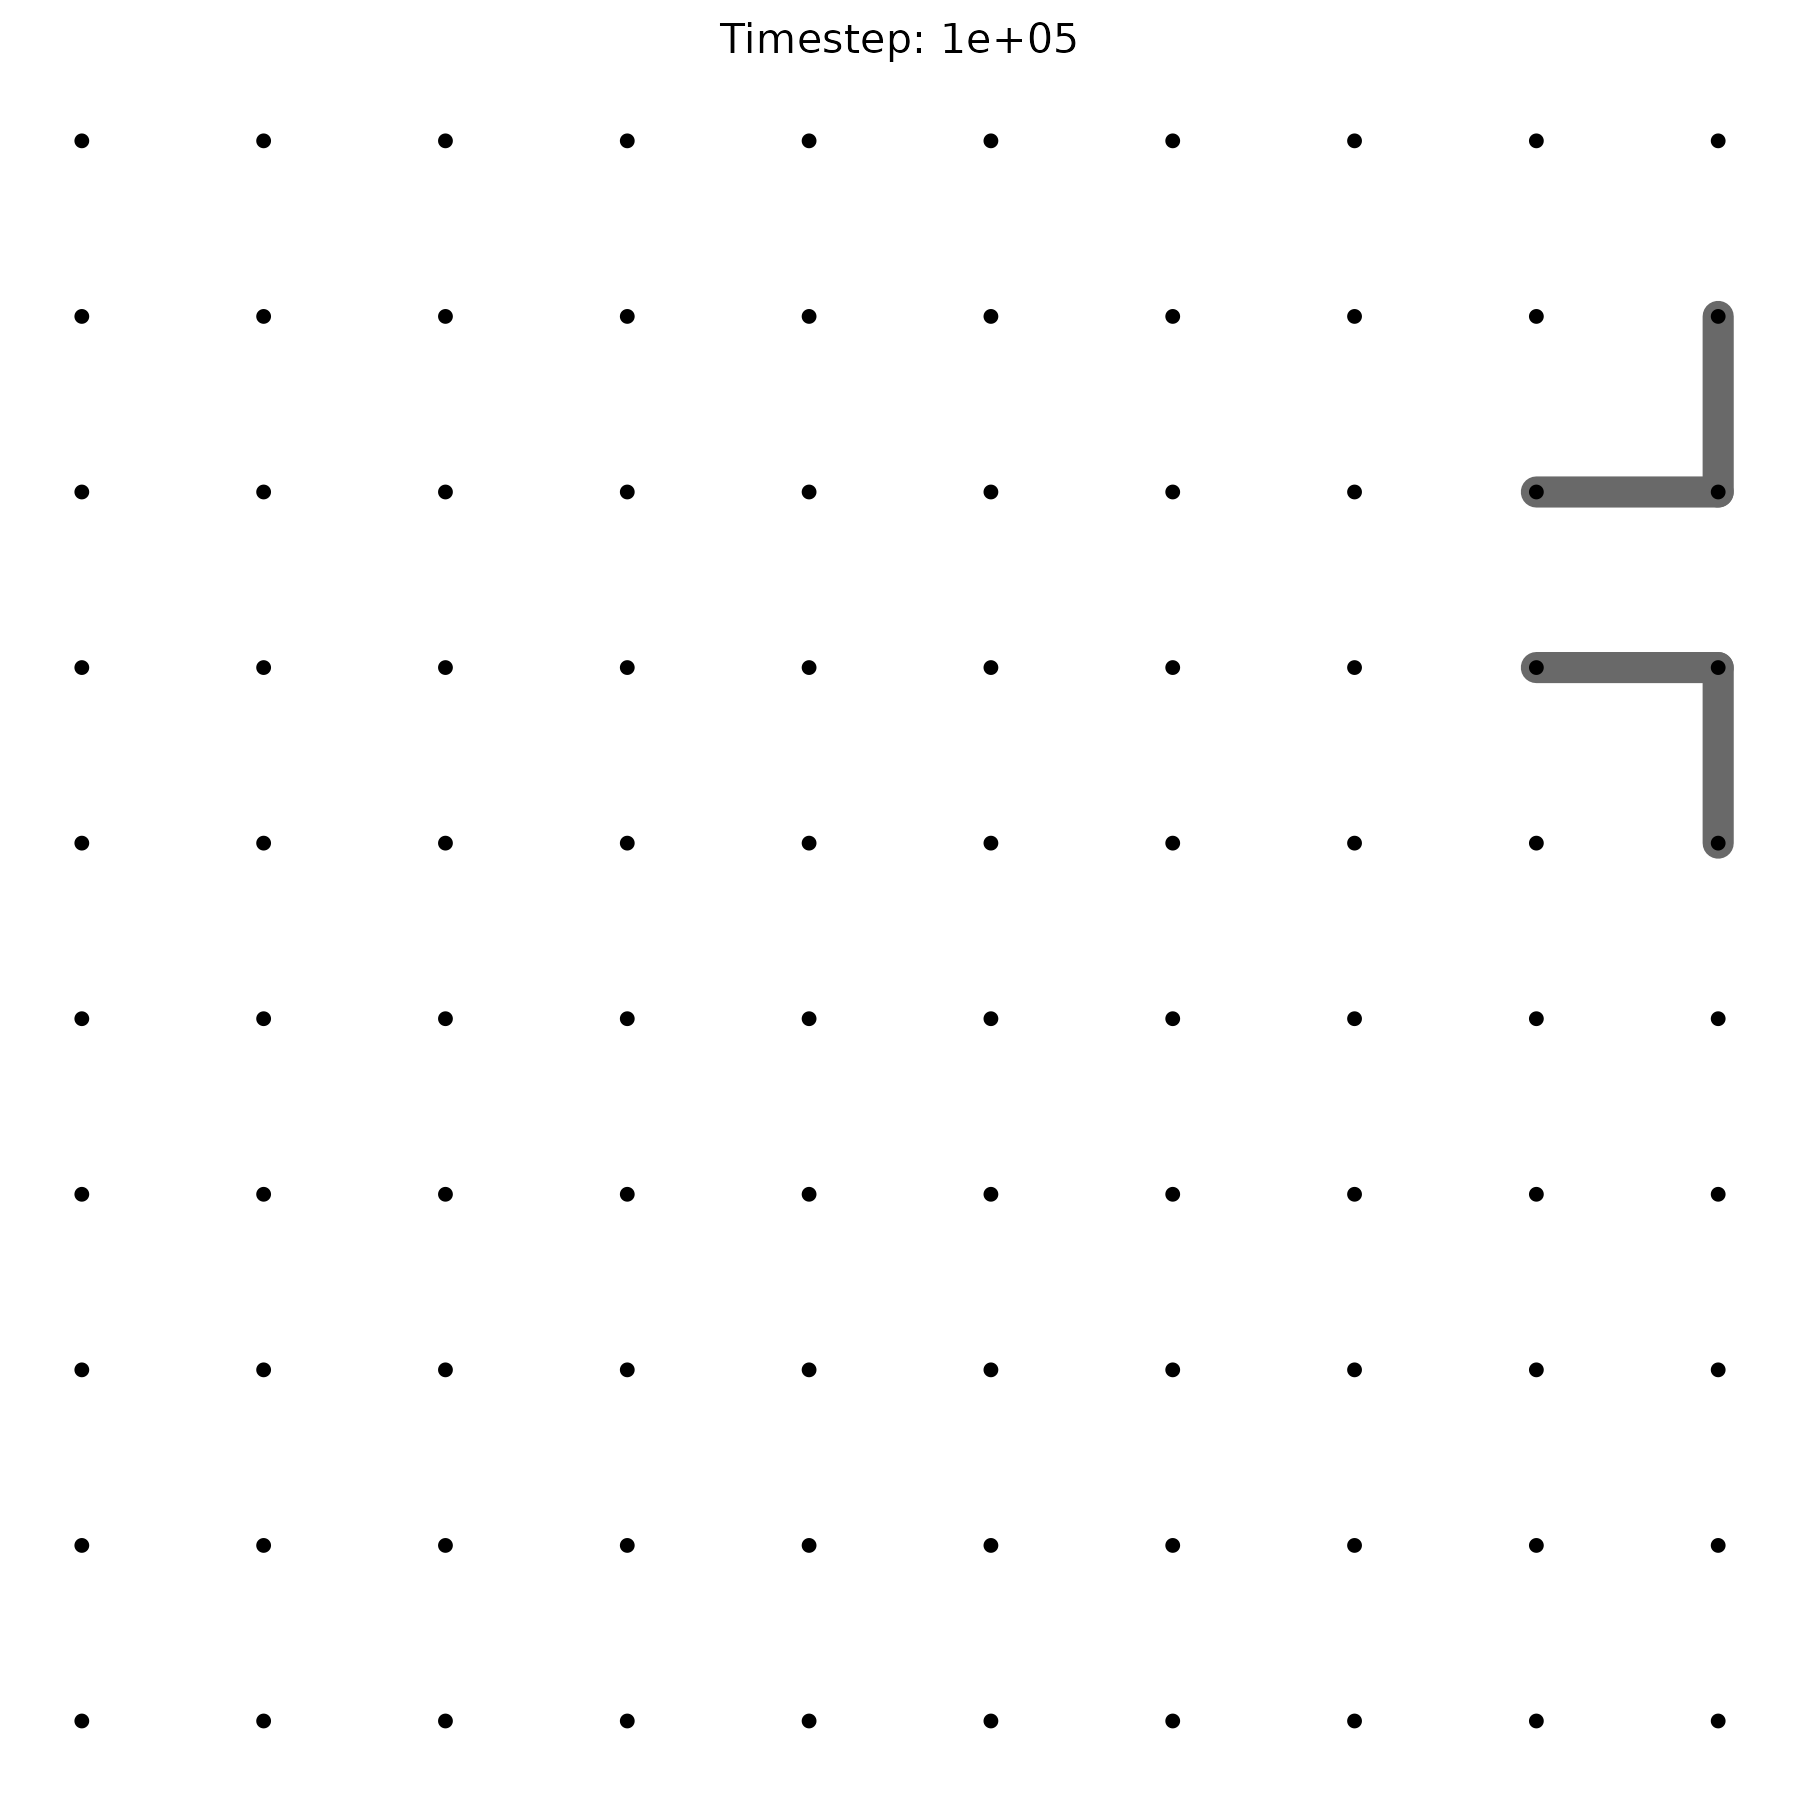
\includegraphics[width=\linewidth]{images/ax3.png}
        
    \end{minipage}
    \caption{Cultural diffusion at several iteration steps. Edges' thickness and darkness are proportional to the dissimilarity among the respective nodes. Timestep is specified on top of the respective figure.}
    \label{fig:ax}
\end{figure}


Such convergence is not guaranteed though, as changing parameters such as the numbers of traits or features may make it significantly less likely to have a single giant connected component. Using table \ref{tab:axsim} as reference, one sees that if the simulation is allowed to run indefinitely until there are no more active sites (i.e. until all sites have either the same culture as their neighbors, or one so different they won't ever interact), certain combination of parameters will results in several distinct cultural regions, thus showing that local convergence may indeed lead to global polarization and to an absence of giant connected component. \\
\begin{table}[h!]
\centering
\begin{tabular}{c@{\hspace{1cm}}ccc}
\multicolumn{4}{c}{\textbf{Average Number of Stable Regions}} \\
\toprule
\multirow{2}{*}{\textbf{Number of Traits}} & \multicolumn{3}{c}{\textbf{Number of Features}} \\
\cmidrule(lr){2-4}
& 5 & 10 & 15 \\
\midrule
5  & 1 & 1 & 1 \\
10 & 2 & 1 & 1 \\
15 & 14 & 2 & 1 \\
\bottomrule
\end{tabular}
\caption{Average number of stable regions per pair of number of traits and features.}
\label{tab:axsim}
\end{table}

\section{Additional topologies}

As noted in the original paper \cite{axelrod_dissemination_1997}, changing neighborhood definitions will induce different convergence tendencies, thus it's likely that changing network topology altogether should also offer alternative insights. The plots below represent the number of cultural regions and active sites (the reason why they are over 100 is because they are recounted depending on how many differing neighbors they have) for the following additional networks:
\begin{itemize}
    \item Barabasi-Albert network (ba): this network  models preferential attachment, in order to show how hubs may accelerate cultural homogenization. The parameters chosen are 1 for the power and 2 for the number of edges to add at each time step.
    \item Watts-Strogatz Small-World Network (ws): this network allows to understand the role of shortcuts in breaking down cultural clusters. Each node is connected to 4 neighbors, with a probability of rewiring of $0.1$.
    \item Stochastic Block Model (sbm): this network that allows to compare for explicit community structure. The graph was partitioned into two equal-sized groups, where nodes of the same community connect with proabability of 90\%, while nodes from different communities connect with probability of 10\%.
\end{itemize}
Plot \ref{fig:models} compares how these models fare against the standard lattice described previously, when setting 5 features and 15 traits. Note that the plot actually takes the average across 10 replications, with the shades around plot lines representing the standard deviation for each model at any specific timestep.
\begin{figure}[htbp]
    \centering
    \begin{minipage}[t]{0.48\linewidth}
        \centering
        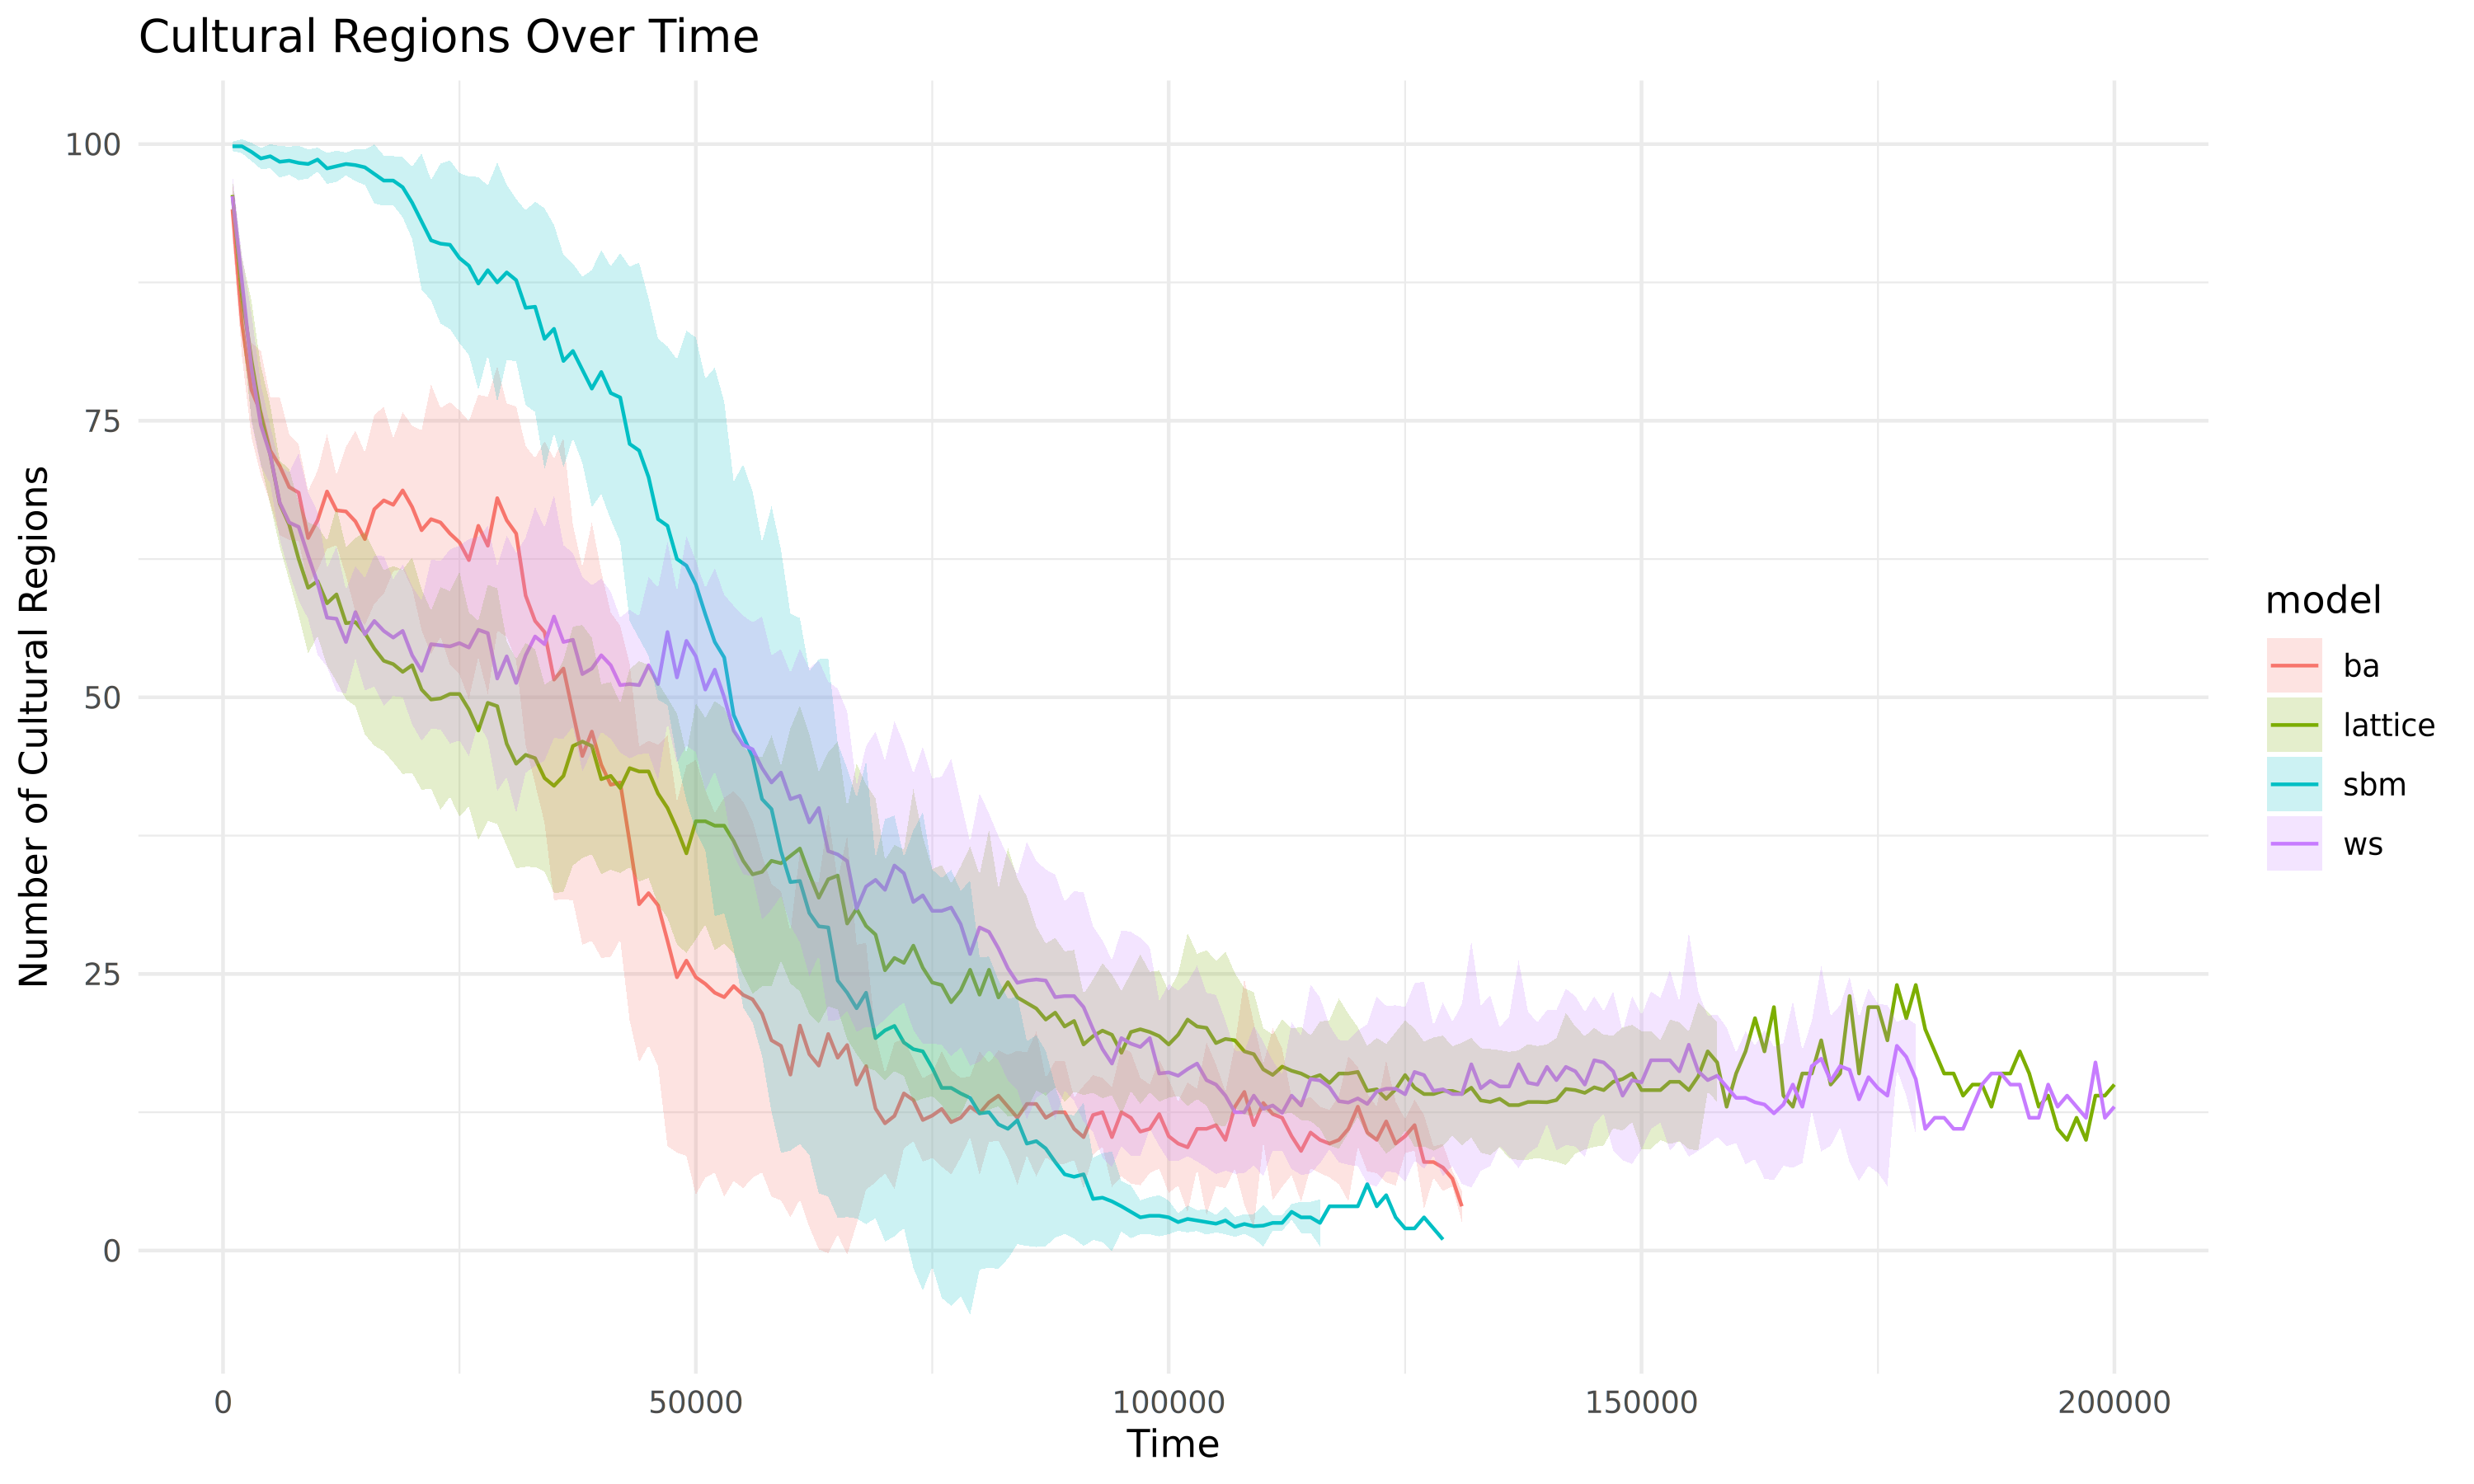
\includegraphics[width=\linewidth]{cultural_regions_over_time.png}
        \caption{Number of cultural regions over time.}
        \label{fig:cultural-regions}
    \end{minipage}
    \hfill
    \begin{minipage}[t]{0.48\linewidth}
        \centering
        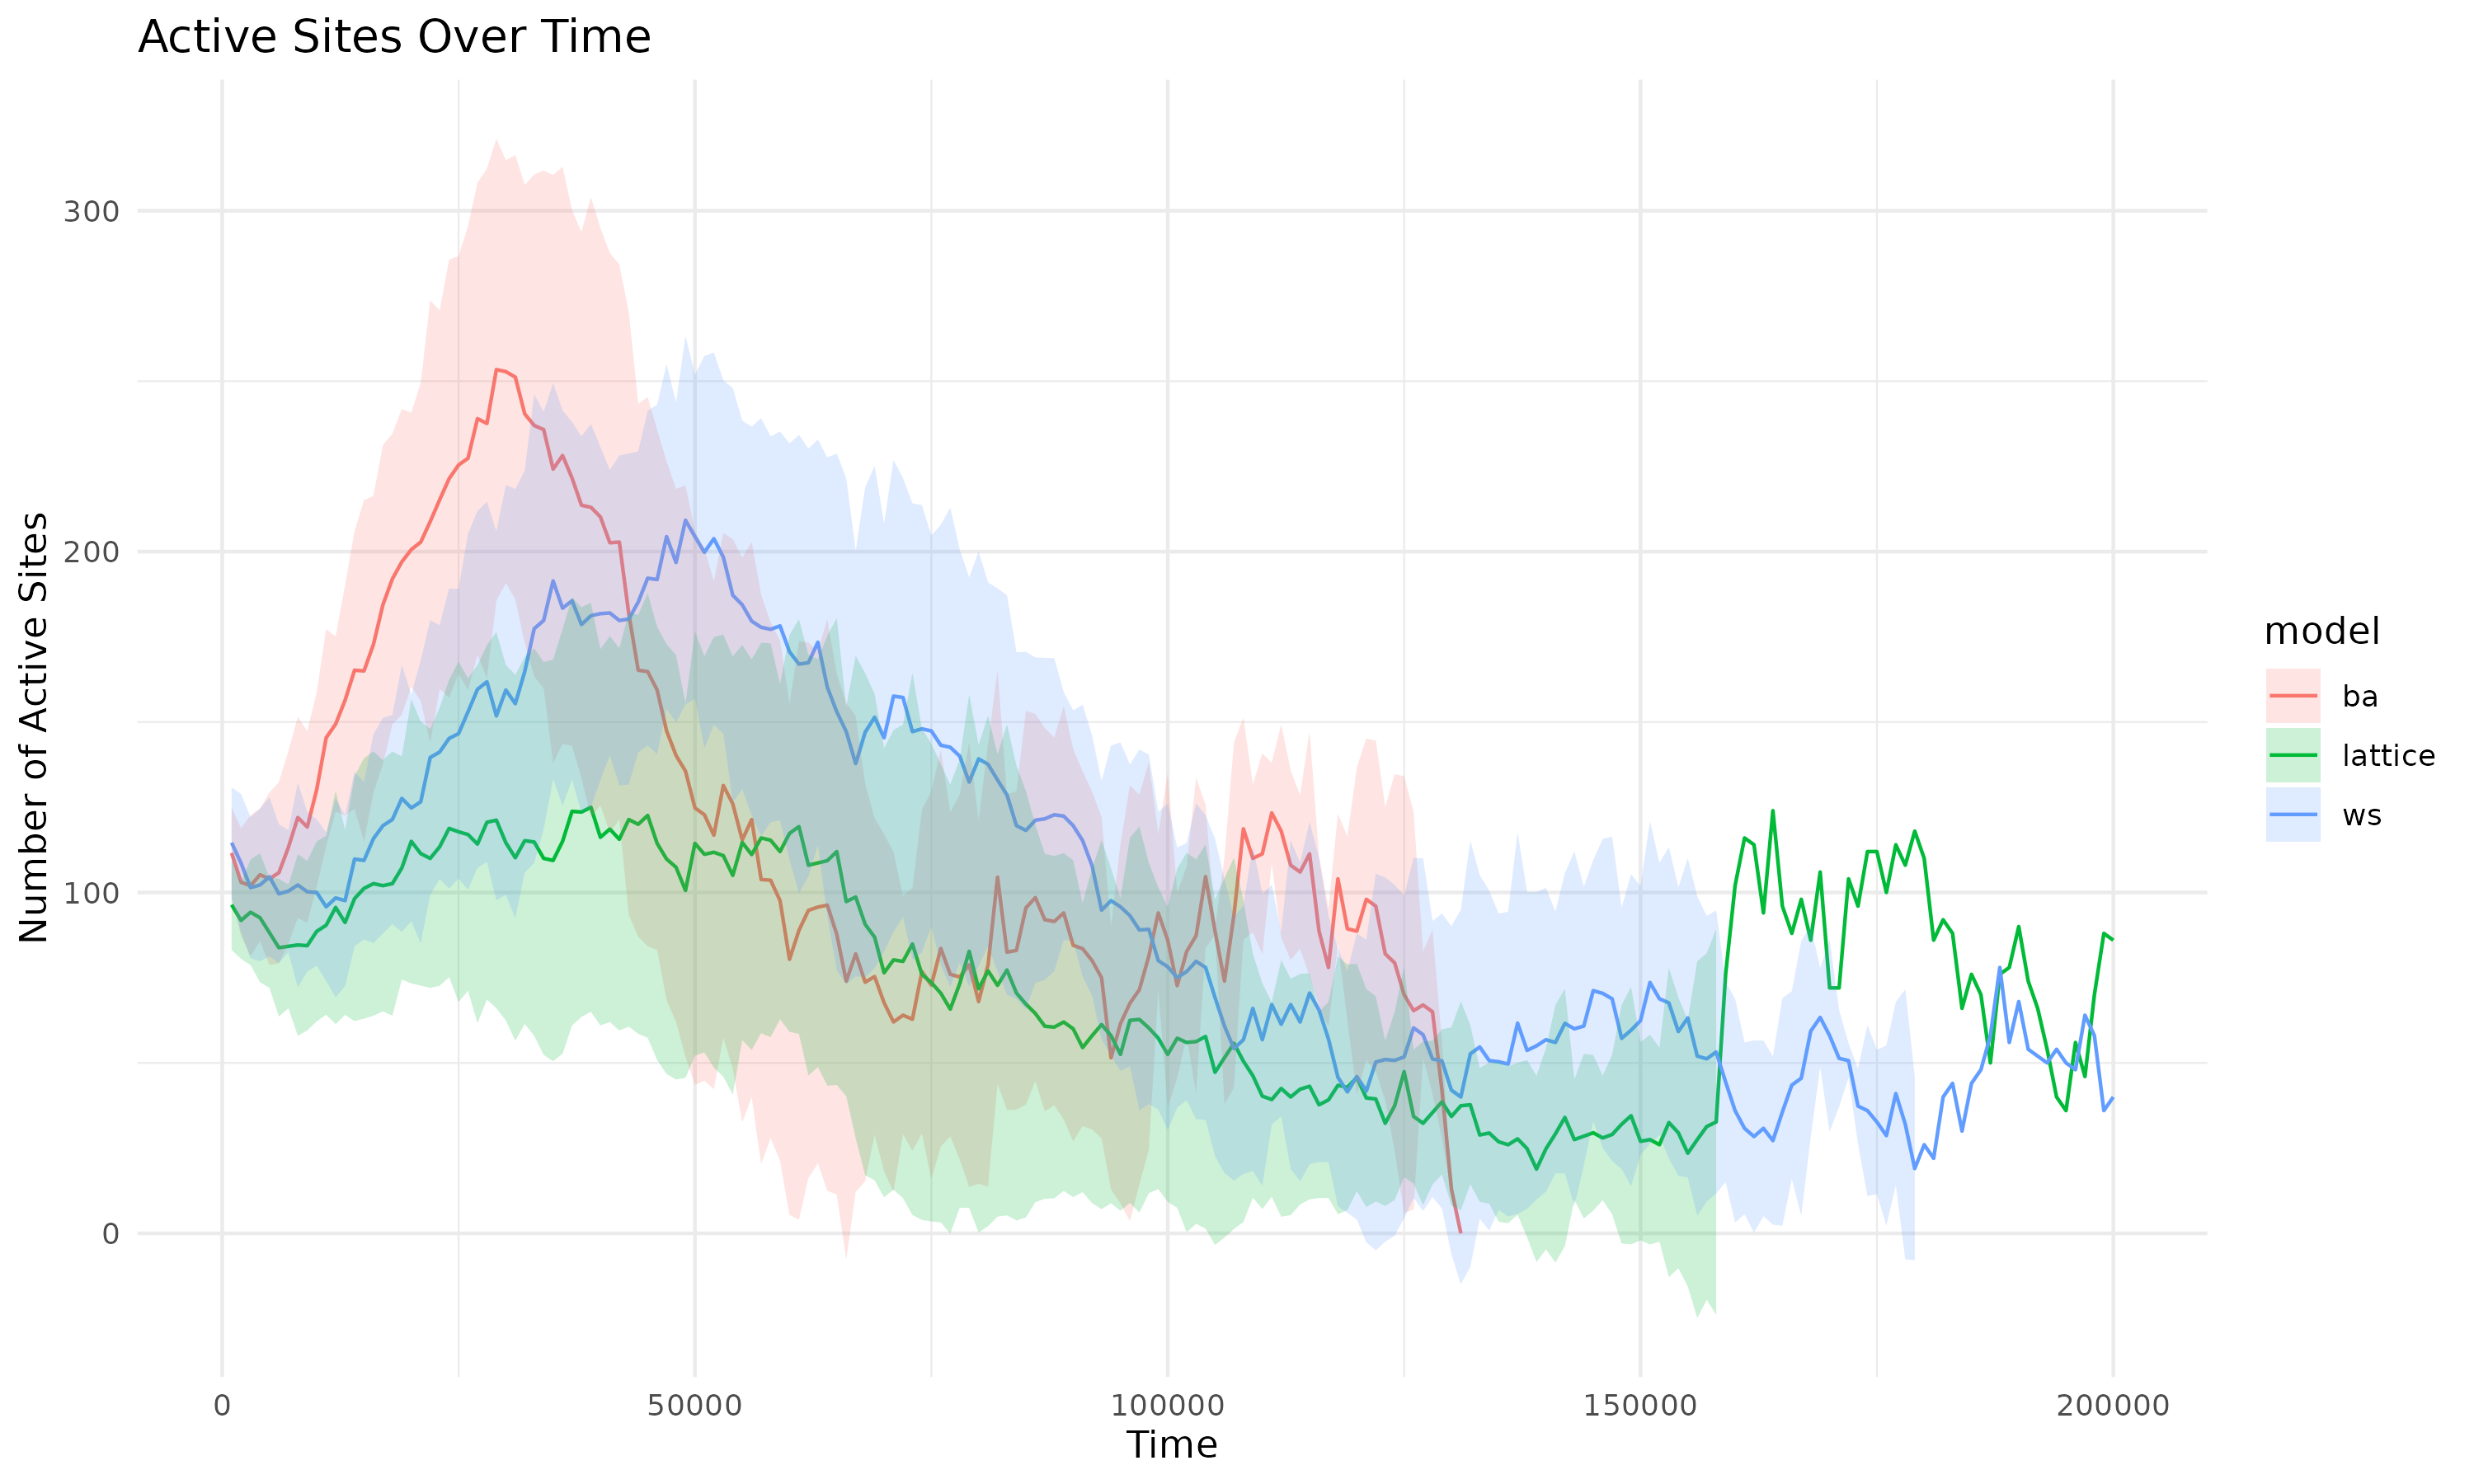
\includegraphics[width=\linewidth]{images/active_over_time.png}
        \caption{Number of active pairs over time. 'sbm' has not been plotted as its number of active sites was too much higher then the rest through the first iterations.}
        \label{fig:active-pairs}
    \end{minipage}
    
    \caption{}
    \label{fig:models}
\end{figure}


As it's clear from the plot, the persistence of multiple cultural regions depends on network structure, which may or may not make it easier for individuals to interact and transmit cultural traits. Interestingly, the SBM tends to be more resistant to homogeneity at first, but then it converges much more quickly.

\newpage